\section{Architecture}
Le système ANPR que nous avons réalisé est essentiellement composé de deux grandes parties:
    \begin{enumerate}
        \item \textbf{Une partie de détection de la plaque}: Dans cette partie, on veut répondre à la question suivante: où se trouve la plaque sur l'image ? En effet, avant de reconnaître le numéro d'immatriculation, il est important de localiser premièrement la position de la plaque sur l'image reçue à travers la caméra. À partir de cette localisation, on peut isoler la plaque du reste de l'image pour l'envoyer à la partie suivante.
        \item \textbf{Une partie de lecture des caractères}: L'entrée de cette partie est la sortie de la partie précédente. L'objectif de cette partie est de reconnaître l'ensemble des caractères sur l'image de la plaque. Cette partie du système retourne alors le numéro du matricule présent sur l'image en format textuel ou ASCII enregistrable dans une base de données.
    \end{enumerate}
    La figure suivante illustre l'architecture que nous avons choisie pour notre système ANPR.
    \begin{figure}[H]
        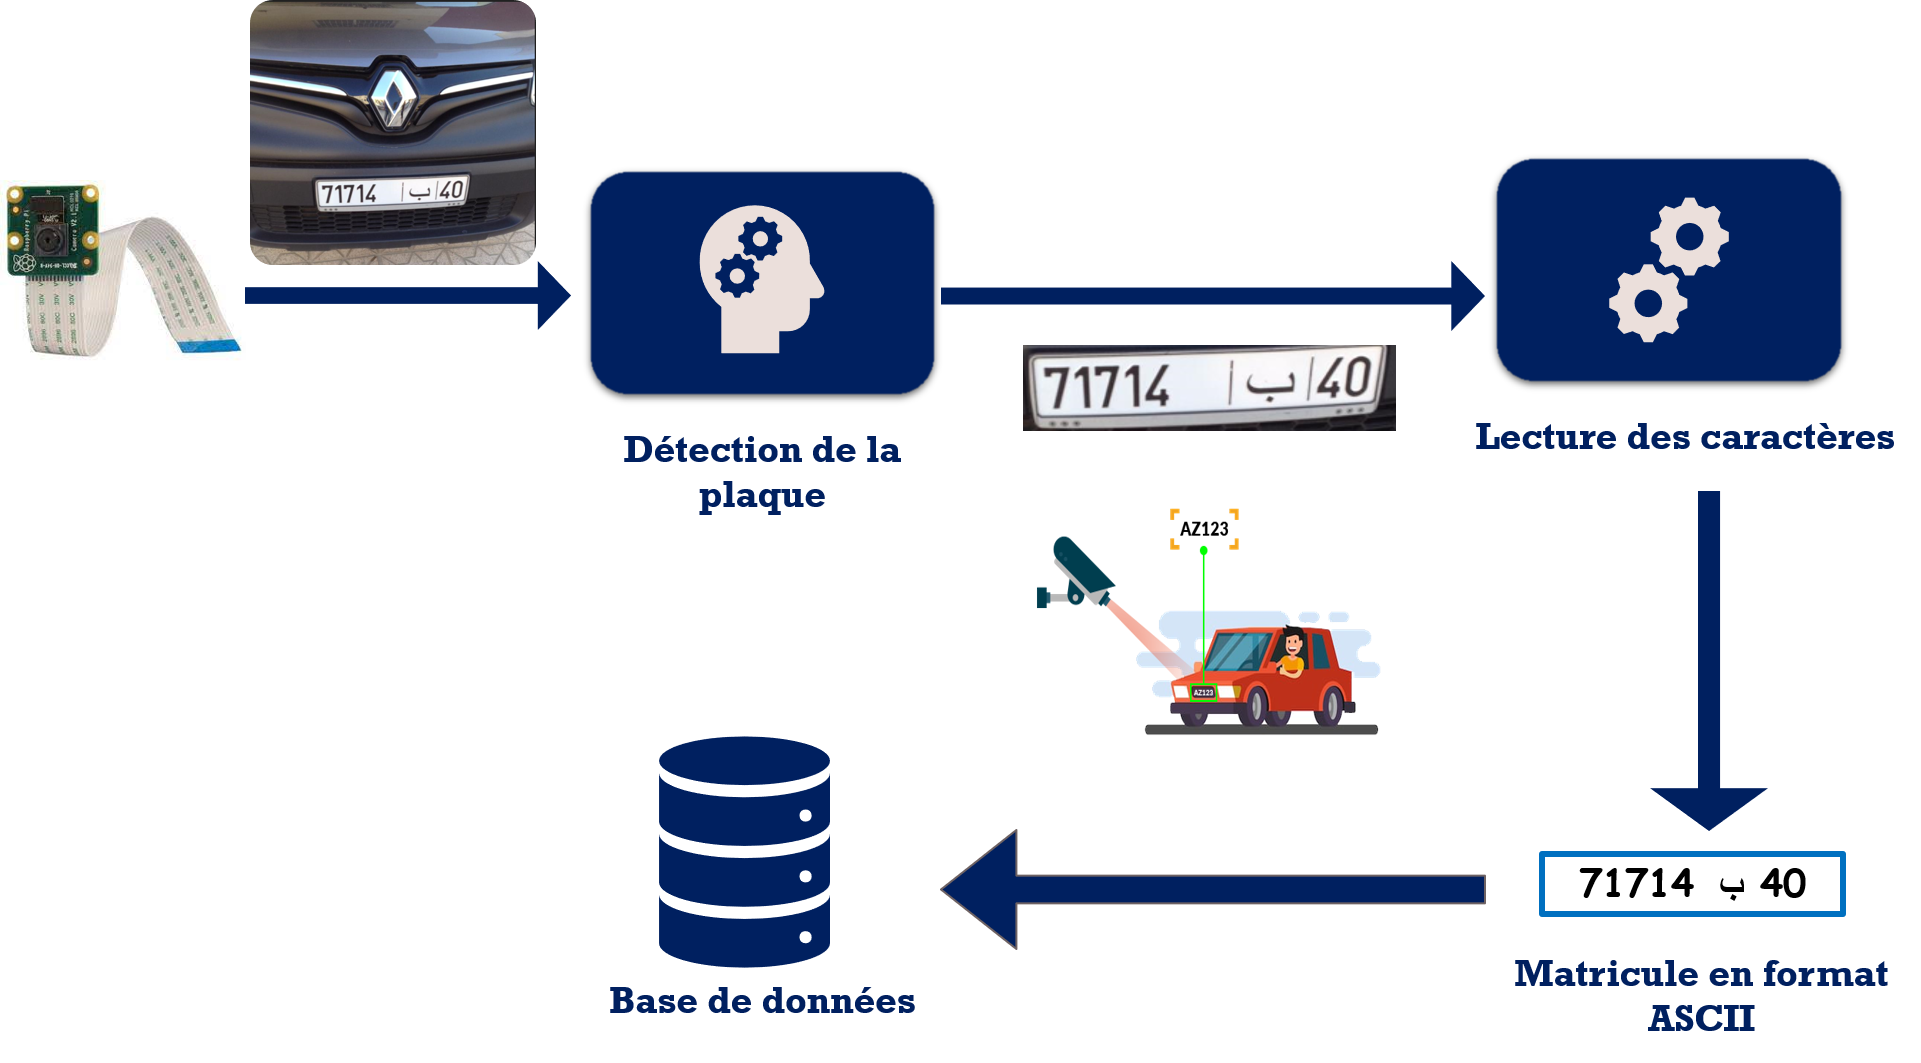
\includegraphics[scale=0.5]{moplazer}
        \caption{Architecture du système MoPlaZer}
    \end{figure}